\documentclass[tikz,border=2pt]{standalone}
\usepackage{amsmath}
\usetikzlibrary{arrows.meta,decorations.pathreplacing}
\begin{document}
% Arrival-time recursion A_k = A_{k-1} + X_k with gaps X = 4, 1, 3, 2: arrival times 4, 5, 8, 10,
% the counting staircase A(t) above them, and A(6) = 2 because A_2 = 5 <= 6 < A_3 = 8.
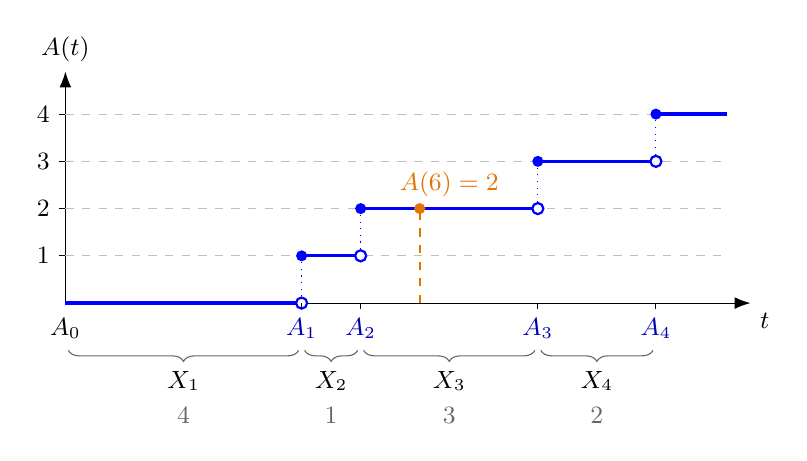
\begin{tikzpicture}[font=\small, >={Latex[length=2mm]}, x=0.75cm, y=0.6cm]
  \draw[->] (0,0) -- (11.6,0) node[anchor=north west] {$t$};
  \draw[->] (0,0) -- (0,4.9) node[anchor=south] {$A(t)$};
  \foreach \y in {1,2,3,4} {
    \draw (0,\y) -- (-0.1,\y) node[anchor=east] {$\y$};
    \draw[gray!50, thin, dashed] (0,\y) -- (11.2,\y);
  }
  % staircase
  \draw[blue, very thick] (0,0) -- (4,0) (4,1) -- (5,1) (5,2) -- (8,2) (8,3) -- (10,3) (10,4) -- (11.2,4);
  \foreach \a/\y in {4/0,5/1,8/2,10/3} {
    \draw[blue, thin, dotted] (\a,\y) -- (\a,\y+1);
    \draw[blue, thick, fill=white] (\a,\y) circle (2pt);
    \fill[blue] (\a,\y+1) circle (2pt);
  }
  % arrival times on the axis
  \foreach \a/\k in {4/1,5/2,8/3,10/4} {
    \draw (\a,0) -- (\a,-0.12);
    \node[blue!70!black, anchor=north] at (\a,-0.12) {$A_{\k}$};
  }
  \node[anchor=north] at (0,-0.12) {$A_0$};
  % gaps as braces below the axis
  \foreach \l/\r/\k in {0/4/1,4/5/2,5/8/3,8/10/4}
    \draw[decorate, decoration={brace, mirror, amplitude=4pt}, gray!80!black]
      (\l+0.05,-1.0) -- node[below=4pt, black] {$X_{\k}$} (\r-0.05,-1.0);
  \node[anchor=north, gray!80!black] at (2,-2.0) {$4$};
  \node[anchor=north, gray!80!black] at (4.5,-2.0) {$1$};
  \node[anchor=north, gray!80!black] at (6.5,-2.0) {$3$};
  \node[anchor=north, gray!80!black] at (9,-2.0) {$2$};
  % reading at t = 6
  \draw[orange!90!black, thick, dashed] (6,0) -- (6,2);
  \fill[orange!90!black] (6,2) circle (2pt);
  \node[orange!90!black, anchor=south] at (6.5,2.05) {$A(6)=2$};
\end{tikzpicture}
\end{document}
